\section{Concept generation and preliminary design}
\subsection{Concept generation}
	With all the premise that lead the development of the project, the first thing that has to be done is generate the concept that can later be compared to choose the best design solution that can become a concrete realization of the ideas.
	
	\paragraph{Kinematic configurations} The first key operation that the robot has to perform is reaching a desired point on the working space and so, in planar kinematics, the machine should present two degrees of freedom that allow to reach all the possible positions; this can be done considering 3 main joint configuration that allows to perform such operations:
	\begin{itemize}
		\item double prismatic joints (figure \ref{fig:kinematiccoupling}.a) where two perpendicular linear guides can be used to move on the plane;
		\item prismatic and revolute joint (figure \ref{fig:kinematiccoupling}.b) where the arm that's free to rotate it's mounted on top of a linear guide. This kind of kinematic chain is currently used by the MindsHub prototype;
		\item double revolute joints (figure \ref{fig:kinematiccoupling}.c), typical configuration of a robot arm, that constraint the framing point to be fixed.
	\end{itemize}
	
	\begin{figure}[bht]
	\centering
		\begin{subfigure}{0.32\linewidth}
			\centering 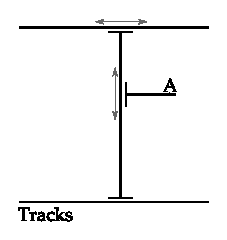
\includegraphics[width=4cm]{kinematics-prism-prism}
			\caption{}
		\end{subfigure}
		\begin{subfigure}{0.32\linewidth}
			\centering 
\includegraphics[width=4cm]{kinematics-prism-rot}
			\caption{}
		\end{subfigure}
		\begin{subfigure}{0.32\linewidth}
			\centering 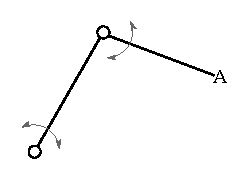
\includegraphics[width=4cm]{kinematics-rot-rot}
			\caption{}
		\end{subfigure}
		\caption{main kinematics coupling that allows to univocally determine the position of a point $A$ in a plane: (a) double prismatic joints, (b) prismatic and revolute joint, (c) double revolute joints.}
		\label{fig:kinematiccoupling}
	\end{figure}
	
	By a first analysis the third configuration (double revolute joint) isn't feasible for the project due to the fact that the system presents a fixed pivot point respect to the frame and to work more area it's mandatory to increase the length of the edges (and this is an issue for the \textit{extendibility} of the machine).
	
	
	

\subsection{Material selection}
	
	The main structural components are beams that, for client requirements, should be standard and so for this reason T slot extruded aluminium profiles (figure \ref{fig:tslot:crosssectionexample}) are chosen after the following considerations:
	\begin{itemize}
		\item better volume-to-price ratio and lower density (respect to inox steels), so reducing costs associated to the spare parts and shipping;
		\item availability in the marker: there are a lot of vendors that provide profiles with various geometrical dimensions, different aluminium alloy and surface finishes. This spare parts can be easily accessed by every private costumer;
		\item for T slot extruded profiles lots of auxiliary components (such supporting brackets, fasteners, hinges...)  are provided from the same profiles manufacturers, reducing the need of custom made part and so decreasing the costs.
	\end{itemize}

	This elements can be also purchased with an anodized finish that allows to improve the corrosion resistance and so increasing the expected life time of the product in uncontrolled outdoor environment.
	
	\begin{SCfigure}[1.5][bh]
		\centering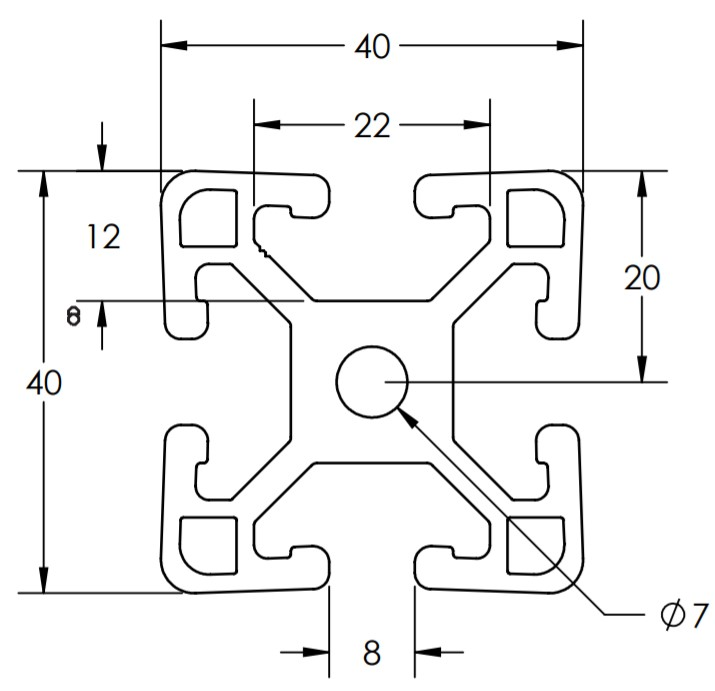
\includegraphics[width=5cm]{tslot-profile-example}
		\caption{technical drawing of a T-slot profile's cross-section. The particular sketch represent the model \texttt{TS40-40LM} by Tslots \cite{tslot-ds}.}
		\label{fig:tslot:crosssectionexample}
	\end{SCfigure}
	
	\paragraph{Mechanical properties} For the design part the following mechanical properties are considered: ultimate tensile strength $\sigma_{uts} = 260 MPa$, yielding strength $\sigma_{ys} = 240 MPa$, Young's module $E = 70 GPa$, Poisson's ratio $\nu = 0.32$; this are mean value and full material designation can be found on table \ref{tab:beammaterial} (page \pageref{tab:beammaterial}).\\
	For the final verification more detailed mechanical properties are going to be used depending on the final profile selection.
	
	
	
	
	
		
	
	
	
	
	
	
	
	
	
	
	
	
	
	
	
	
	
	
	
	
	
	
	
	
	
	
	
	
	
	
	
	
	
	
	
	
	
	
	
	
	
	
	
	
	
	
	
	
	
	
	
	
	
	
	
	
	
	
	